\chapter{Interpretation of Results}
\label{chap:upper_limit}

No events were observed in data that satisfies the signal selection, and the result is consistent with the SM expectations. Therefore, upper limits (ULs) are set on the cross section times branching ratio ($\sigma \times$ BR) for resonances decaying to a dilepton.

\section{Statistical Procedure}
The limits are calculated using \textit{HistFitter v0.61.0}~\cite{Baak:2014wma}, a statistical tool used for limit settings in ATLAS. The limit setting procedure is based on the modified Frequentist method, \CLs~\cite{OBRAZTSOV1992388,PhysRevD.57.3873}. In this framework, a number of events, $n$, is modeled as a Poisson distribution with the mean $\lambda = \mu_{\mathrm{sig}}\cdot s + b$ where $\mu_{\mathrm{sig}}$ is the signal strength parameter. The systematic uncertainty estimated in Chapter~\ref{chap:syst} is introduced as the nuisance parameter $\theta$ to $s$ and $b$, i.e. $s$ and $b$ become a function of $\theta$. The method uses the LHC default one-sided profile likelihood ratio $q_{\mu_{\mathrm{sig}}}$ as a test statistic,

\begin{equation}
q_{\mu_{\mathrm{sig}}} = -2 \log \Bigg( \dfrac{L(n_\mathrm{obs}~|~\mu_{n_\mathrm{sig}}, \Hat{\Hat{\theta}})}{L(n_\mathrm{obs}~|~\Hat{\mu}_{\mathrm{sig}}, \Hat{\theta})}\Bigg)
\label{eq:test_statistic}
\end{equation}
%
where $L$ is the likelihood function, $\Hat{\mu}_{\mathrm{sig}}$, $\Hat{\theta}$ are the values that globally maximize the likelihood, $\Hat{\Hat{\theta}}$ is the value that maximizes the likelihood for the specific value of $\mu_{\mathrm{sig}}$, and $n_{\mathrm{obs}}$ is the observed number of events in data or in pseudo experiments.

The distributions of the test statistic $q_{\mu_{\mathrm{sig}}}$ for the signal + background and background hypothesis ($\mu_{\mathrm{sig}} = 1$ or $\mu_{\mathrm{sig}} = 0$) are obtained from multiple pseudo experiments, and the Frequentist probability (or $p$-value) is calculated from the distributions as,

\begin{align}
\mathrm{CL}_{s+b} = P(q_{\mu_{\mathrm{sig}}} > q_{\mu_{\mathrm{sig}}}^{\mathrm{obs}}~|~\mu_{\mathrm{sig}} = 1), \nonumber \\
\mathrm{CL}_{b} = P(q_{\mu_{\mathrm{sig}}} > q_{\mu_{\mathrm{sig}}}^{\mathrm{obs}}~|~\mu_{\mathrm{sig}} = 0),
\label{eq:p_values}
\end{align}
%
where $\mathrm{CL}_{s+b}$ is the probability to obtain a test statistic value more extreme than the observed test statistic, $q_{\mu_{\mathrm{sig}}}^{\mathrm{obs}}$, assuming signal + background hypothesis ($\mu_{\mathrm{sig}}=1$), and $\mathrm{CL}_{b}$ is the corresponding probability for background hypothesis. Using these confidence levels, the signal confidence level, \CLs, is defined as
\begin{align}
\CLs =  \dfrac{\mathrm{CL}_{s+b}}{\mathrm{CL}_{b}}.
\label{eq:cls}
\end{align}

The UL at the 95\% confidence level are obtained by adjusting $\mu_{\mathrm{sig}}$ until \CLs reaches 0.05, and the limit is translated to the $\sigma \times$ BR by the relation,

\begin{equation}
\label{eq:signal_strength}
\mathcal{L}_{Int.} \cdot \big(\sigma \cdot \mathrm{BR} \big) \cdot \epsilon = \mu_{\mathrm{sig}}\cdot s + b,
\end{equation}
%
where $\mathcal{L}_{Int.}$ is the integrated luminosity and  $\epsilon$ is the signal efficiency.

\section{Upper limits}
The observed ULs are evaluated by performing pseudo experiments with an expected background of 0.27$\pm$0.14 events, the systematic uncertainty of 10\%, and the uncertainty of the luminosity measurement of 2.2\%.

The observed ULs at 95\% CL on $\sigma \times$ BR for $Z' \rightarrow$ \mumu, \ee, and \emu are shown in Figure~\ref{fig:upper_limits} as a function of $c\tau$. The observed limits are relatively uniform in $c\tau$ for all channels. At $m_{Z'}=$ 1 TeV, the ULs are from 0.5 - 0.9 fb. At $m_{Z'}=$ 100 GeV, the ULs are much larger (50 - 400 pb) than other mass points due to the limited trigger efficiency.


\begin{figure}[!htb]
    \centering
    \subfloat[]{\label{subfig:ul_mumu}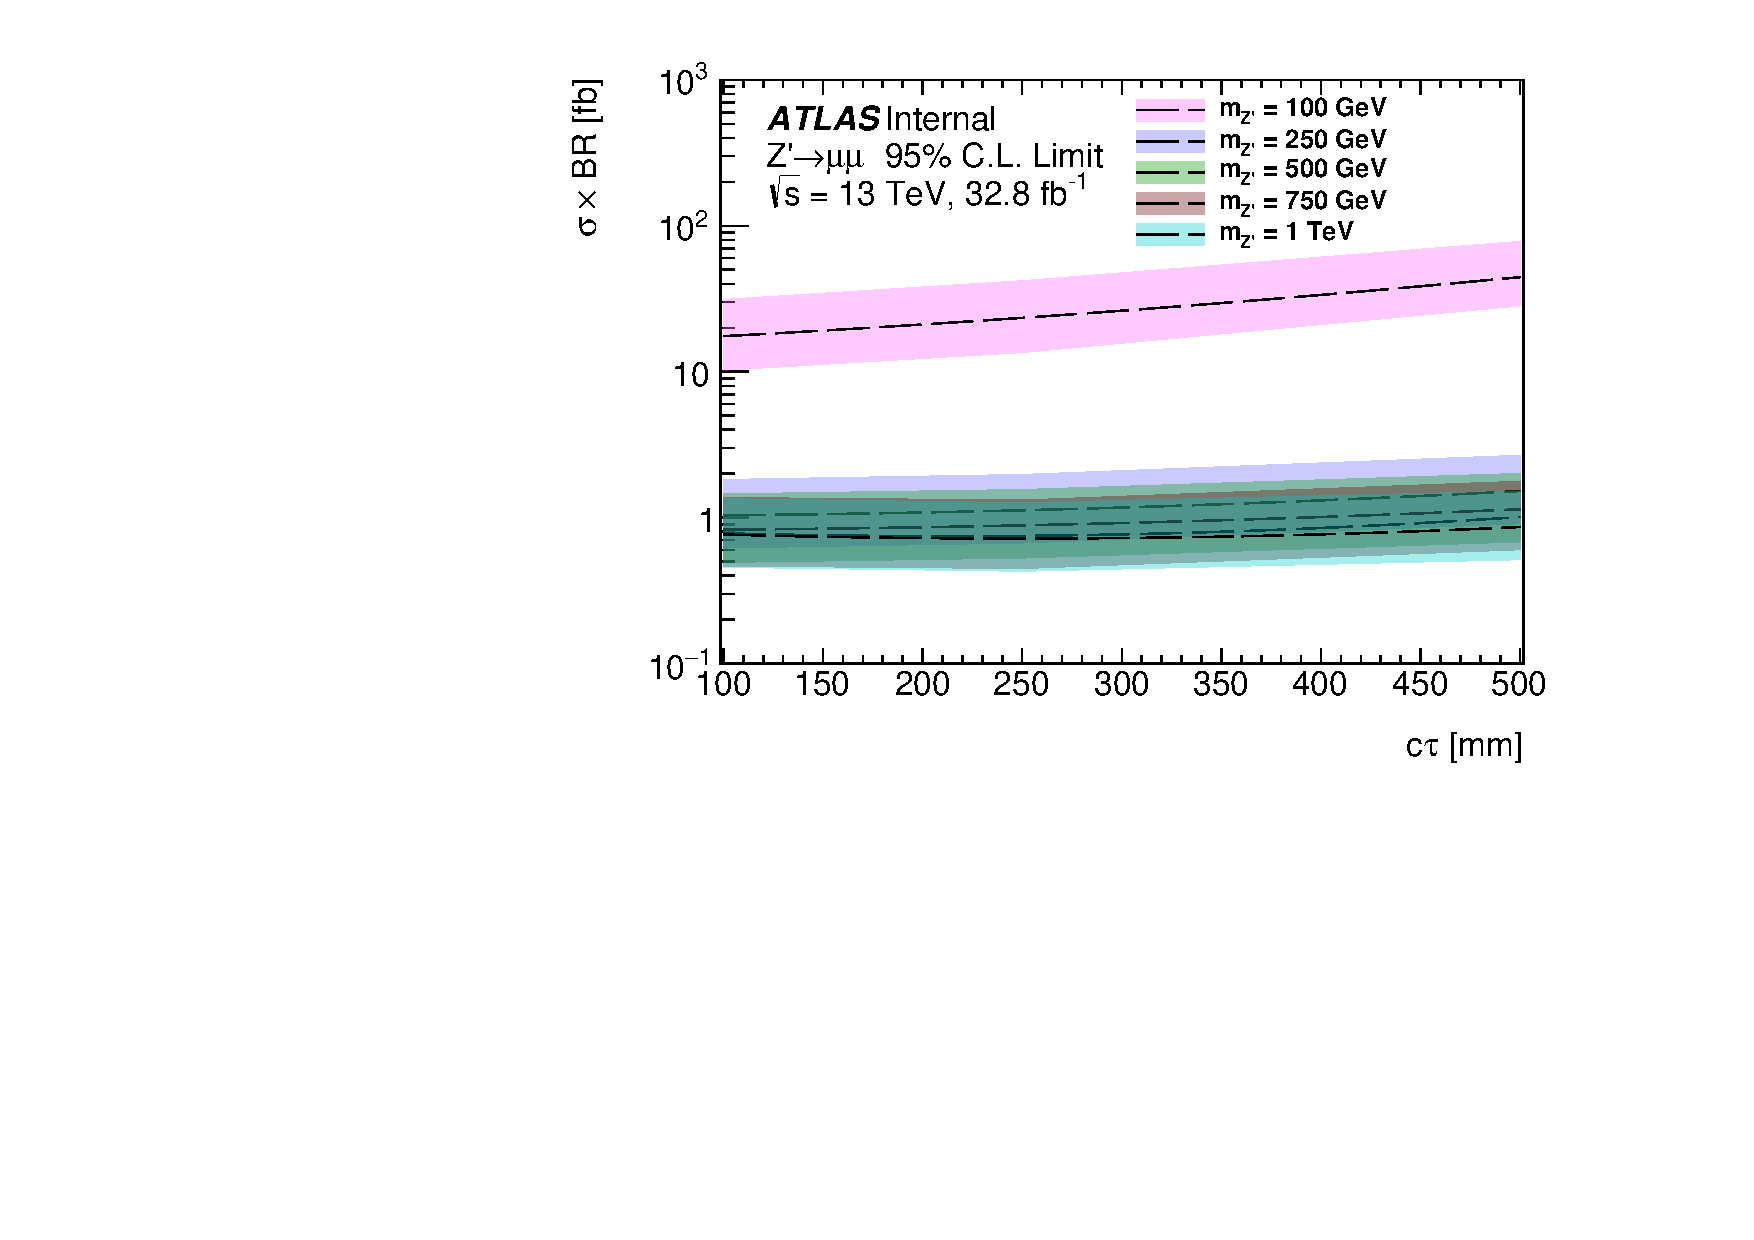
\includegraphics[width=0.60\textwidth]{figures/UL/DiMu_UL.pdf}} \\
    \subfloat[]{\label{subfig:ul_ee}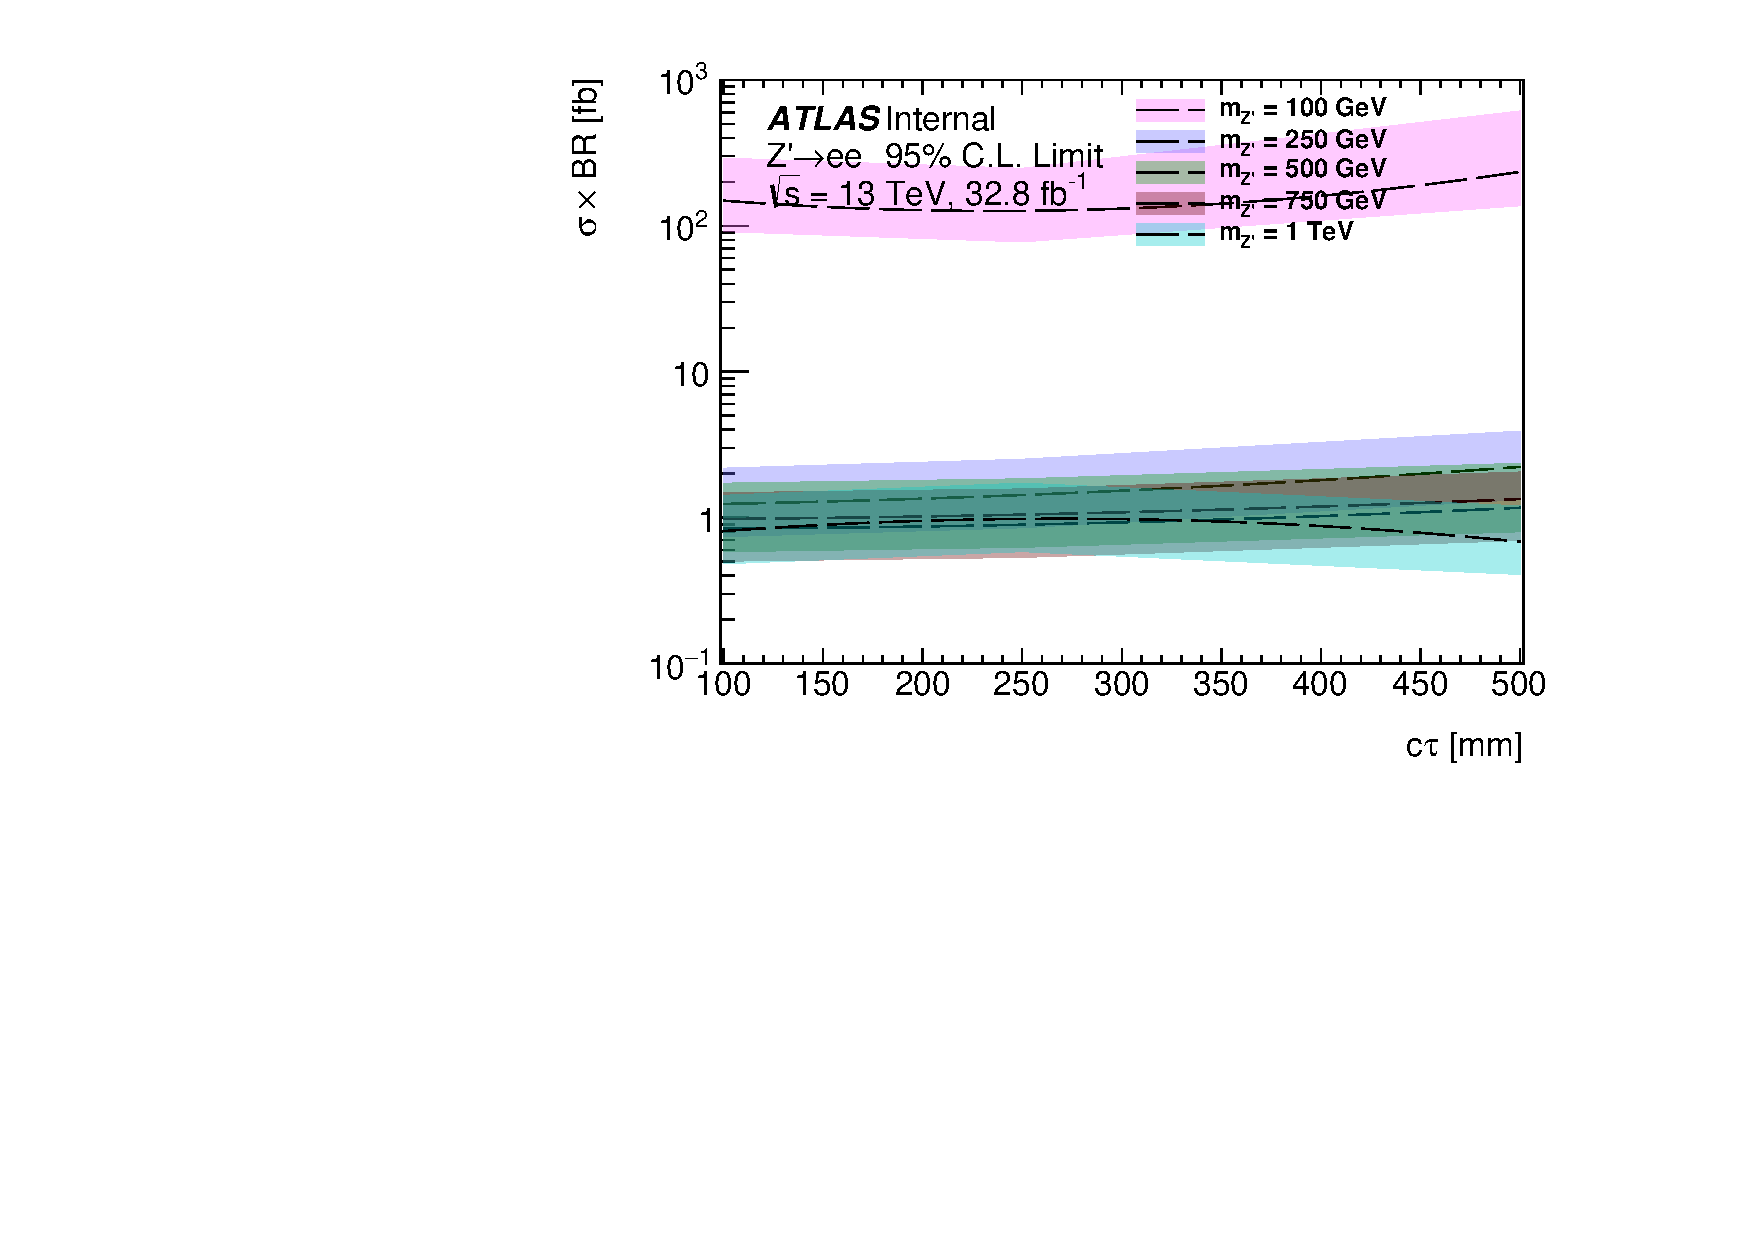
\includegraphics[width=0.60\textwidth]{figures/UL/DiE_UL.pdf}}    \\
    \subfloat[]{\label{subfig:ul_emu}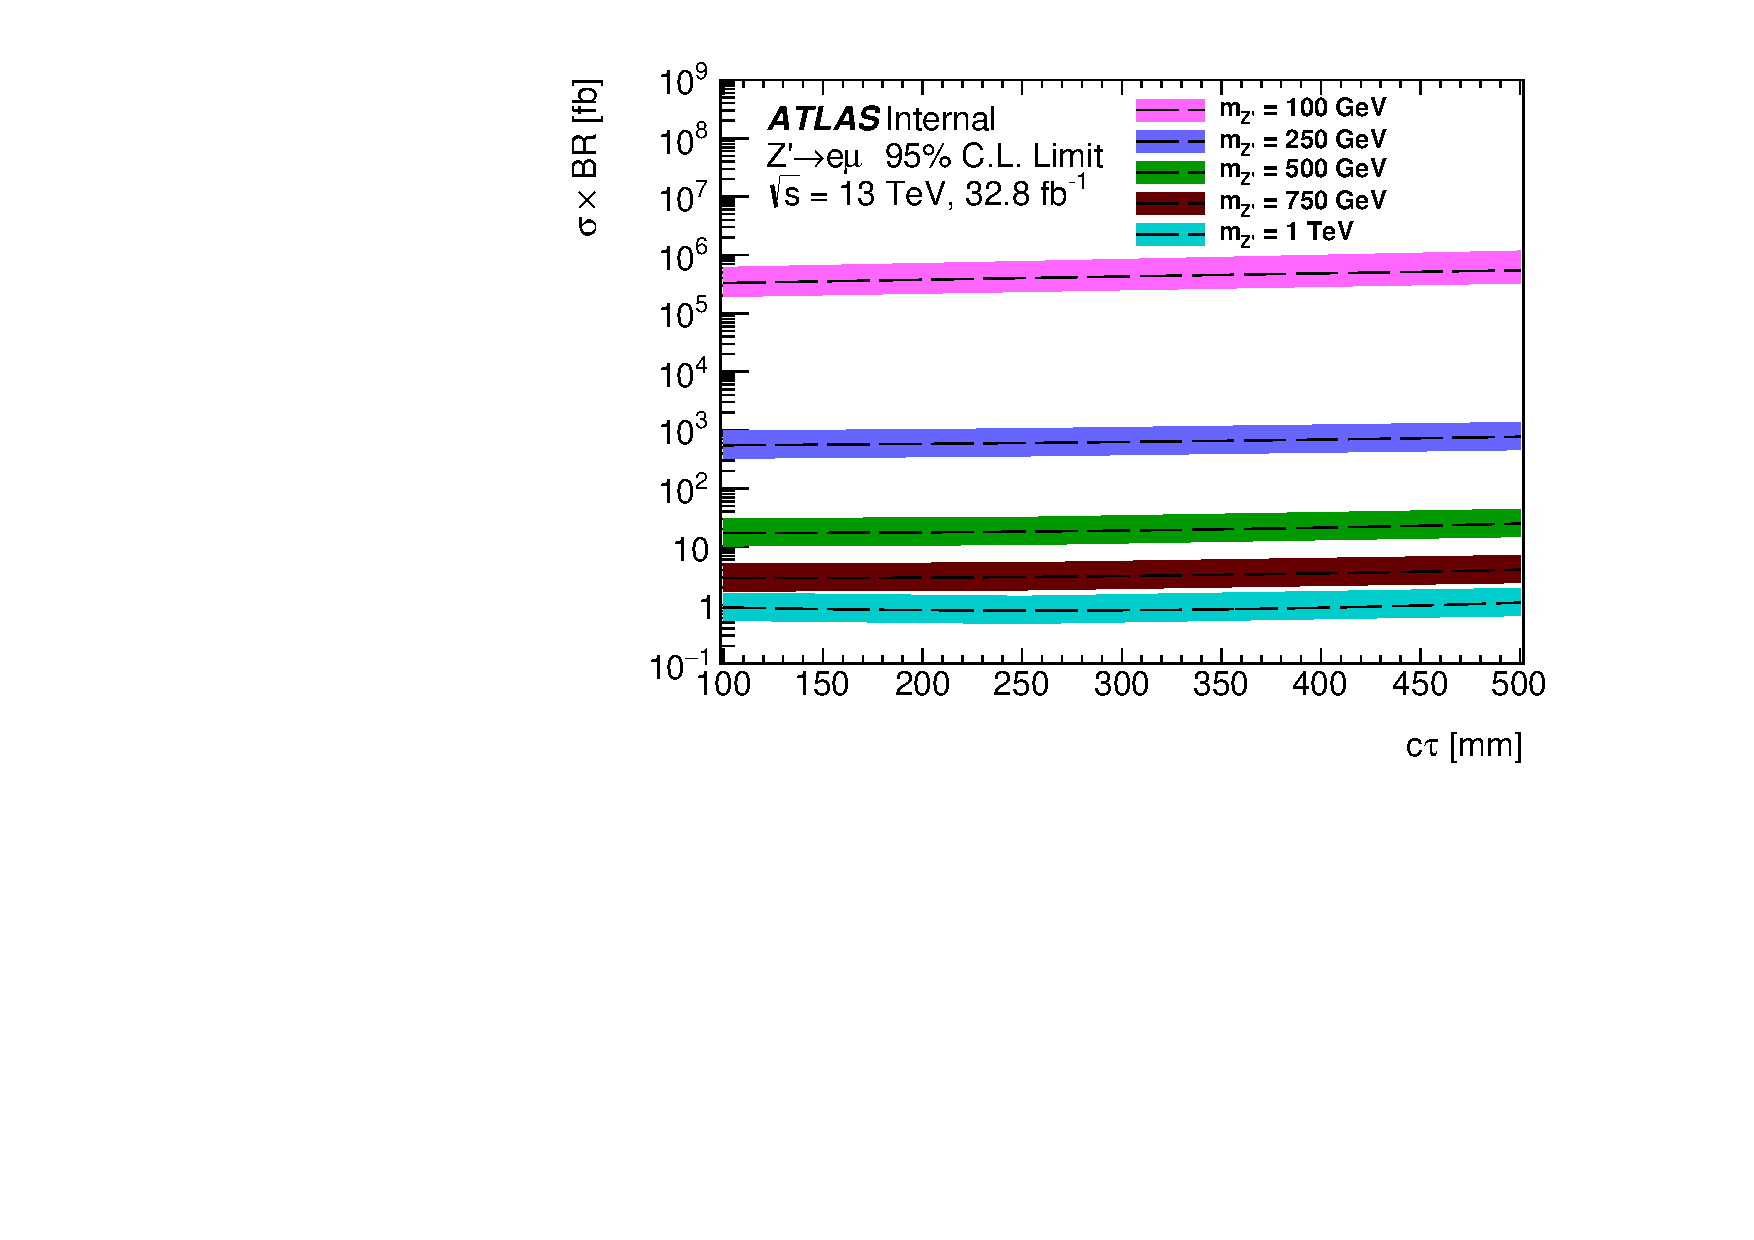
\includegraphics[width=0.60\textwidth]{figures/UL/EMu_UL.pdf}}   \\
    \caption{The observed 95$\%$ CL upper limits on the $\sigma \times$ BR for the $Z'\rightarrow$ (a) \mumu, (b) \ee, and (c) \emu signal samples with $Z'$ masses of 100 - 1000 GeV as a function of $c\tau$. The dashed lines are expected limits, and the solid bands represent 1$\sigma$ uncertainty on the expected limit.}
    \label{fig:upper_limits}
\end{figure}

